\subsection{M.PC.RI - Rischi Inattesi}

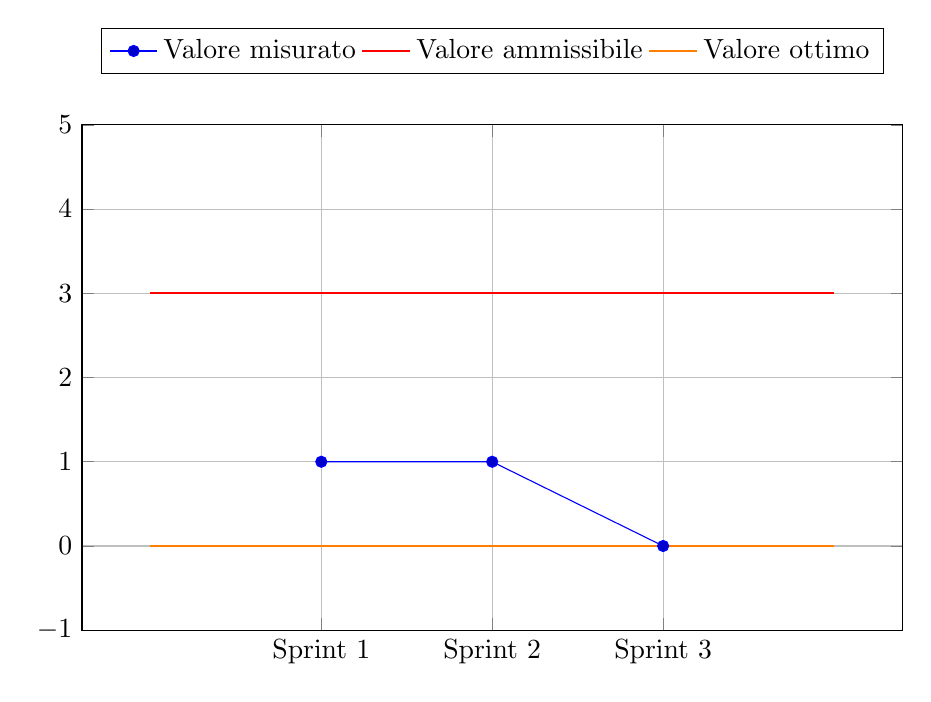
\begin{tikzpicture}
    \begin{axis}[
        width=12cm, height=8cm,
        ymin=-1, ymax=5,
        xtick={1, 2, 3},
        xticklabels={Sprint 1, Sprint 2, Sprint 3},
        xlabel={},
        ylabel={},
        grid=major,
        scaled ticks=false,
        legend style={at={(0.5,1.1)}, anchor=south, legend columns=-1},
    ]
    \addplot coordinates {(1, 1) (2, 1) (3, 0)};
    \addlegendentry{Valore misurato}
    \addplot[red, thick] coordinates {(0, 3) (4, 3)};
    \addlegendentry{Valore ammissibile}
    \addplot[orange, thick] coordinates {(0, 0) (4, 0)};
    \addlegendentry{Valore ottimo}
    \end{axis}
\end{tikzpicture}

\subsection*{RTB}

\subsection*{PB}